% [CS 6210] Project 3 Writeup
% Authors: Anish Khale, Nikita Gupta

\documentclass[11pt,pdftex,twocolumn]{article}

\usepackage{epsf}
\usepackage{epsfig}
\usepackage{url}
\usepackage{ifthen}
\usepackage{comment}
\usepackage{fancyhdr}
\usepackage[margin=1in]{geometry}
\usepackage{setspace}
\usepackage{abstract}
\usepackage{lipsum}
\usepackage{amsmath}

\renewcommand{\headrulewidth}{0.4pt}
\renewcommand{\footrulewidth}{0.4pt}
\pagestyle{fancy}
\lhead{\bfseries CS 6210 : Spring 2014}
\chead{\bfseries Project 3}
\rhead{\bfseries March 27, 2014}
\renewcommand{\abstractnamefont}{\normalfont\normalsize\bfseries}
\renewcommand{\abstracttextfont}{\normalfont\small}
\setlength{\absleftindent}{0pt}
\setlength{\absrightindent}{0pt}
\title{RPC Based Proxy Server}
\author{
Anish Khale\\
\url{anish_khale@gatech.edu}
\and
Nikita Gupta\\
\url{ngupta71@gatech.edu}
}
\date{}

\begin{document}
\maketitle
\fancyfoot{}
\fancyfoot[C]{\thepage}
\thispagestyle{fancy}

\begin{abstract}
Remote Procedure Calls (RPC) are powerful, commonly-used abstractions for constructing distributed applications. One such modern RPC technology is Apache Thrift. Thrift allows for scalable, cross-language services development by combining a software stack with a code generation engine to build services that work efficiently and seamlessly between C++, Java and a host of other languages. Caching in a distributed system environment further helps to improve efficiency of accessing the required data. In this project, we combine the powerful abstraction of RPC from Apache Thrift with the efficiency and high performance of various caching schemes in a distributed application.
\end{abstract}

\section{Introduction}
% Intro explains briefly what you built, what you measured, and what you found from your experiments. Conclusion should reiterate this, with more weight on the conclusion you reach from your experiments.
To build a RPC-based proxy server, a modular approach was taken beginning with generating a C++ server skeleton code using Apache Thrift. Next, the ability to make curl requests, using the \texttt{libcurl} library, was added to this server to fetch the HTML content from a particular website pointed to by its URL, passed as a parameter by a requesting client over RPC. Having the RPC portion of the project taken care of, we built in the code libraries for caching policies that included Random Eviction, First In First Out (FIFO) and Least Recently Used (LRU) as the cache replacement policies. Sections~\ref{sec:cacheDesign} and~\ref{sec:cachePol} explain these cache designs and policies, respectively, in detail.

To measure the performance of the three caching policies, two performance metrics were selected, viz. hit ratio and average memory access time, and are described in detail in section~\ref{sec:perfMetrics}. Experiments were run under two different workload patterns, as described in section~\ref{sec:perfWork}, and the experimental setup and methodology is described in detail under section~\ref{sec:exp}. Results obtained from these experiments indicate that the decision of choosing the right cache replacement policies has a significant performance impact on cache performance. The results, documented in section~\ref{sec:results} and analysed in section~\ref{sec:analysis}, prove that under varying workloads, LRU performs the best while the performance obtained from random eviction of cache entries is the least.

\section{Task Division}
% Who did what.
The tasks associated with this project can be broadly classified into three main categories: Code, Test and Documentation. The breakdown of tasks along with the team members they were assigned to respectively are shown in table~\ref{tab:taskDiv}.
% Table for section 2
\begin{table*}[t]
\centering
\begin{tabular}{| c | p{3.5in} | c | c |}
\hline
Category & Task & Anish K. & Nikita G.\\
\hline\hline
& RPC using Apache Thrift & 100\% & 0\%\\
\cline{2-4}
& Fetching HTML from URL using \texttt{libcurl} & 100\% & 0\%\\
\cline{2-4}
& Random Eviction policy & 0\% & 100\%\\
\cline{2-4}
Code & FIFO policy & 0\% & 100\%\\
\cline{2-4}
& LRU policy & 0\% & 100\%\\
\cline{2-4}
& Test Harness & 50\% & 50\%\\
\cline{2-4}
& Integration & 100\% & 0\%\\
\hline
Test & Integration & 50\% & 50\%\\
\cline{2-4}
& Performance & 50\% & 50\%\\
\hline
Documentation & Writeup & 50\% & 50\%\\
\hline
\end{tabular}
\caption{Task Division for Project 3}
\label{tab:taskDiv}
\end{table*}

\section{Cache Design}
% Clearly explains the operations the cache supports, the data structure(s) used, and the algorithms that implement the cache operations. (Note: no need to explain how standard data structures or algorithms work, e.g., "linked list" or "linear search" can be named without further explaination)
\label{sec:cacheDesign}
Generally application developers want to reduce expensive operations and, therefore, wish to reuse some results to improve application performance. Hence caching comes into play. In caching, pages referred by the user are stored in a cache, so when the same page is requested it can be restored from the cache instead of going to the main memory and fetching that page. This saves time and improves performance of the application. 
\begin{figure}[!h]
\centering
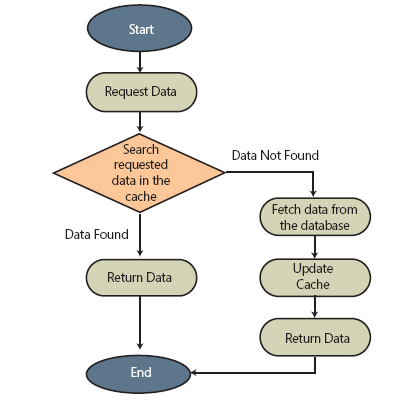
\includegraphics[scale=0.6]{images/cache.PNG}
\caption{Working of a cache based system}
\label{img:cache}
\end{figure}
In this project cache memory is used to store copies of web pages to exploit localities of reference. When client requests a web page, server first checks the presence of web page in the cache, if present it will fetch the web page and send it to the client. If not present, the server gets the web page from the internet, updates the cache entry and sends it to the client. So, in this project, a web cache is implemented at the server which stores URLs which have been accessed by the client. Implementing this caching policy reduces time that the server takes to process clients request if it is a cache hit, if it is a cache miss normal time is taken to get the web page from the internet. This will in turn improve application performance. The URL and data are stored in a Key-value container, key being the URL and value being the HTML present in that URL.
\begin{figure}[!h]
\centering
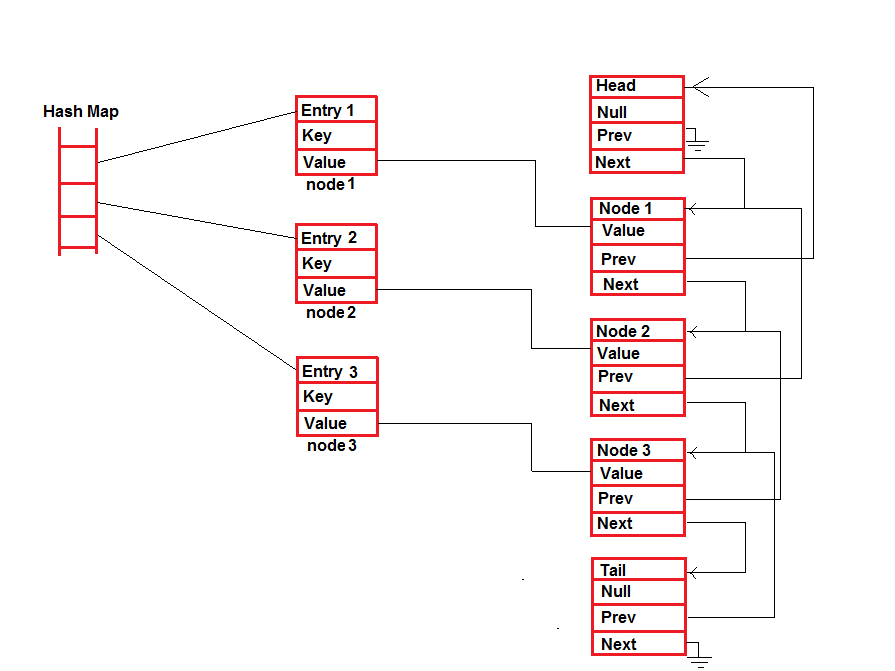
\includegraphics[scale=0.35]{images/cache_impl.png}
\caption{Cache implementation}
\label{img:cache_impl}
\end{figure}
Cache implementation, in this project, is done using hashmap and doubly linked list, as shown in fig~\ref{img:cache_impl}. Hashmap stores Key-Value pairs and doubly linked list is used to index the pairs in order of data age. There are two functions which are implemented one is \texttt{search\_cache()} and the other is \texttt{insert\_into\_cache()}. These two functions are self descriptive by their names. When client request a URL server calls \texttt{search\_cache()} to find the URL in the cache, if it is present, it is a hit else a miss. In case of hit the URL content is returned to the client, in case of miss server searches for that URL on the internet and updates the cache entry and returns the content to client. For updating cache entry \texttt{insert\_into\_cache()} function is called. First this function checks whether the size of cache is big enough to add new entry or not. If memory is available to add new entry life is good, else using a cache replacement policy one of the entry is removed and in place of that new entry is added. Hashmap is used for storing key-value pairs and searching in hashmap is O(1) which is very efficient, hence making the caching algorithm efficient.

\section{Caching Policies}
% Each of three cache policies is described clearly, describing how evictions are chosen and what the good & bad points of such a policy are. The reader should understand well enough to replicate these cache policies.
\label{sec:cachePol}
One of the important factors in selecting an effective caching policy is the lifetime of the resource. In order to store a new resource in cache, an existing cache resource needs to be swapped out if the cache becomes full; this is known as paging. There are different paging algorithms, viz., LRU(Least Recently Used), LFU(Least Frequently Used), FIFO(First In First Out), MRU(Most Recently Used). Caching policy is selected with the goal to minimize paging and maximizing cache hits. In this project, we have implemented Random, FIFO and LRU cache replacement policies.
\subsection{Random}
In Random paging an entry is selected at random to be evicted. When client requests a web page and entry is not present in the cache and cache size is full, then randomly a entry is selected and that entry is evicted. In case of cache hit, the entry is returned to the client and no change in the cache is done. While in the case of cache miss, randomly selected entry is deleted from the doubly linked list.
\subsubsection{Pros}
\begin{itemize}
	\item Searching complexity is O(1) because to search the entry hashmap is used.
	\item Deletion complexity is O(n), where n is the random number which is generated using \texttt{rand()}. While loop is implemented which iterates till n and then that entry is evicted, hence complexity is O(n).
\end{itemize}
\subsubsection{Cons}
\begin{itemize}
	\item In this policy a pseudo random number generator is required, In this project we are using a standard C++ \texttt{rand()} function.
	\item This policy makes no attempt to benefit from temporal or spatial localities. 
	\item Cache is not thread safe, i.e cache is not safe for concurrent modifications, when multiple clients call the same server.
\end{itemize}

\subsection{First In First Out (FIFO)}
In this paging policy, the page which has been in the cache the longest is evicted, i.e the page which was stored in the cache first gets swapped out first. So to implement this policy we have maintained a queue using doubly linked list. New cache entries are added at the end of the queue and entries to be deleted are deleted from the staring i.e head of the queue. Whenever an entry is present in the queue and is requested by the client, then server returns the entry as a response to the client request and no change is made in the queue.
\subsubsection{Pros}
\begin{itemize}
	\item Search complexity of this algorithm is same as that of random algorithm, O(1).
	\item Deletion complexity is O(1), because entry which is at the head of the doubly linked list is evicted.
	\item This algorithm tries to take benefit from temporal locality of cache.
\end{itemize}
\subsubsection{Cons}
\begin{itemize}
	\item It requires more space, as queue is used to maintain First In First Out policy.
	\item Cache is not thread safe, i.e cache is not safe for concurrent modifications, i.e when multiple clients call the same server.
\end{itemize}

\subsection{Least Recently Used (LRU)}
When cache capacity is full and new content needs to come in, the previous content has to be swiped out to make space for new content. In LRU known as Least Recently Used, the content which is not used since a long duration of time i.e the content which has been used the least will be replaced. Thereby making space for new content. In this project we have implemented LRU as the third caching policy. In the doubly linked list new cache entry is added at the front of the list just after the head, so this makes the end or tail of the list as the least recently used entry. So when an entry has to be deleted the last entry is deleted and the new entry is added at the head of the list. Now if the entry is already present in the cache and is requested by the client, then this entry is deleted from that position and the entry is again added to the front of the list, making it the most recently used entry. In this way LRU policy is implemented.
\subsubsection{Pros}
\begin{itemize}
	\item Searching complexity of this algorithm is O(1), which is also the complexity of FIFO and Random. 
	\item Deletion complexity is O(1), because every time the entry at the end of the doubly linked list is evicted.
\end{itemize}
\subsubsection{Cons}
Cache is not thread safe, i.e cache is not safe for concurrent modifications, i.e when multiple clients call the same server.

\section{Performance Evaluation Metrics}
% The chosen metrics for evaluation are described clearly, so it is easily understood what each metric represents and measures, and a justification is given for why each metric was chosen. Chosen metrics accurately reflect how "good" the cache policies they measure are. The reader should understand well enough to use these metrics him/herself and get comparable results.
\label{sec:perfMetrics}
The chosen metrics for evaluating the performance of the three caching policies detailed in the previous section are indicative of the time saved by not having to access the memory and the correctness of the policies in having those pages in the cache that fulfil a very high number of URL requests coming in.
\subsection{Hit ratio}
Hit ratio ($h$) is a basic performance metric that measures the ratio of the number of memory references that hit in the cache and the total number of memory references.
Mathematically,
\newline
\begin{equation}
\label{eq:h}
h = \left(\frac{hits}{hits + misses}\right)
\end{equation}
This metric was chosen because it can accurately indicate the number of times a request, that is made, can  be found in the cache (a hit) versus the number of times it has to be served by fetching the data from the physical memory. Ideally, the highest value possible for $h$ is 1. Practically, higher the value of $h$, the better the concerned caching policy is.
\newline
An equivalent performance metric is Miss ratio ($m$), where,
\begin{equation}
\label{eq:m}
m = (1 - h)
\end{equation}
\subsection{Average memory access time}
The average memory access time ($t_{avg}$) accurately conveys the amount of time the server spends in the cache to serve an incoming request versus that spent to access the same from the main memory. It is computed as
\begin{equation}
t_{avg} = \left(h * t_{cache} + m * t_{memory}\right)
\end{equation}
where,
$h$ and $m$ are calculated as per equations (\ref{eq:h}) and (\ref{eq:m}) respectively, and $t_{cache}$ and $t_{memory}$ are the times required to access the cache and main memory respectively. Lower the value of $t_{avg}$, better is the particular caching policy.

\section{Performance Evaluation Workloads}
% Each of two workloads is described clearly, so it is easily understood how each workload is generated. The reader should understand well enough to replicate these workloads. (Note: the exact list of URLs used is not needed; the pattern in which they are accessed is what matters)
\label{sec:perfWork}
To obtain the most accurate results from the performance evaluation of the caching policies, we choose the following two patterns of workload distribution, assuming four URLs: A, B, C and D. In our experiments, we include these patterns directly in their individual text files such that the URLs can be individually read by the client. 
\subsection{Workload 1: Uniform Distribution}
There is no fixed order of querying URLs in this workload. The pattern signature can be depicted as BDADACAABCBBADDABCD$\ldots$.
\subsection{Workload 2: Statistical Distribution}
In this distribution, each unique URL is queried a specific number of times consecutively. The pattern signature can be depicted as ABBCCCCADDDDBBCCCA$\ldots$.

\section{Experimental Setup and Methodology}
% The experimental methodology is described clerly, including machines used, how they are networked, the software run, what was measured and how, and the procedures used. A hypothesis is given regarding which policies will and won't work well on each workload, with justification for that belief. (Note: it is not necessary for these hypotheses to match the actual results, as long as the discrepency is discussed in the analysis; it's okay for hypothese to be wrong!)
\label{sec:exp}
The experimental setup for this project includes two laptops, one running the client on a 32-bit version of Ubuntu with 3 GB RAM and the other running the server and hosting the cache on a 64-bit version of Ubuntu with 8 GB RAM. Both devices consist of Intel's quad core i5 processor and are networked to each other via a common WiFi interface over port 8080.

As discussed in section~\ref{sec:perfMetrics}, we evaluate the performance of the three caching policies by measuring the hit ratio and the average memory access time for the caches on the server machine. We write a test harness that includes a set of two URL list files, one for each workload, on the client that it makes request to the server from, and a code on the server to measure the aforementioned parameters for each workload.

Based on the workload patterns described in section~\ref{sec:perfWork}, we hypothesize that, with the cache present in our experiments, the random eviction policy should perform better for workload 1 since there is no predictable pattern of querying URLs to the server, while LRU should perform better for workload 2 due to the doctored pattern signature. In either case, the no-cache policy should yield equivalent results. The actual results of this experiment are documented in the graphical format in section~\ref{sec:results}.

\section{Results}
% Experimental results are presented using graphs that show the chosen metrics vs. the cache size. Results are given for each policy running against each workload. Graphs are presented in a clear an legible manner, with a descriptive title/caption, labeled axes (including unit labels), scales, distinguishable lines (on mult-series graphs), and a legend (on multi-series graphs). (Note: no need to present any raw data; the graphs are sufficient - if you want to include raw data, do so in a separate file, not in the writeup)
\label{sec:results}
\lipsum[1]

\section{Analysis of Results}
% All features on the presented graphs are identified and described clearly. An explaination is given for each feature on the graphs.
\label{sec:analysis}
\lipsum[1]

\section{Conclusion}
As expected the experiment showed the same results. OMP barriers are faster than MPI barriers. Tournament barrier has the least execution time, it reduces contention and spinning of processes is pre determined unlike rest barriers. Tree barrier reduces contention but still can suffer from contention if the value of K is large. Sense Reversal barrier faces lots of contention as spinning is on same memory location for same shared variable.
\end{document}